\mychapter{Exames com MCTest+Moodle+VPL}\label{ch:examesQT_VPL}

Neste capítulo, serão descritos exames que contêm questões dissertativas (QTs) paramétricas, nas quais os estudantes devem submeter exercícios de programação (EPs) em atividades VPL do Moodle. Esses tipos de questões foram detalhados na Seção \ref{sec:questoesQT_VPL} -- \nameref{sec:questoesQT_VPL}. A questão de parcelas sem juros criada nesta seção será utilizada em um novo exame, no qual será detalhado todo o processo neste capítulo.

Esse tipo de exame tem sido amplamente utilizado na UFABC em disciplinas que envolvem programação, como Bases Computacionais da Ciência (equivalente à CS0 -- \textit{Computer Science} 0), para estudantes ingressantes. Nessa disciplina, a linguagem de programação Python é empregada juntamente com a biblioteca \verb|pandas|, permitindo que os estudantes pratiquem estatísticas em arquivos no formato CSV.

Outra disciplina que faz uso frequente dessa integração com o \textit{plugin} VPL é a de Processamento da Informação (PI), equivalente à CS1 (\textit{Computer Science} 1). CS1 representa a primeira disciplina introdutória em Ciência da Computação, geralmente oferecido no primeiro ano de graduação em cursos dessa área. A definição CS1 foi estabelecida pela ACM (\textit{Association for Computing Machinery}), uma das principais associações profissionais de Ciência da Computação do mundo \cite{hogan2023cs0}.

Ao longo dos anos, diversos professores da UFABC têm contribuído para o desenvolvimento de questões, resultando em um total de 2.516 questões cadastradas até janeiro de 2024. Dessas questões, 691 são do tipo paramétricas, como indicado em \href{http://mctest.ufabc.edu.br/}{mctest.ufabc.edu.br}.

É importante destacar que, embora essa metodologia de avaliação seja adotada em diversas turmas, muitos professores ainda não utilizam essa abordagem ou outras similares. Isso pode indicar uma falta de padronização dos conteúdos apresentados aos estudantes, o que pode prejudicar o processo de ensino-aprendizagem, com detalhado por \citeonline{2018:Zampirolli.Goya.ea}.

Todo o processo de criação de exames descrito nos capítulos anteriores pode ser aplicado a exames que utilizam a integração do VPL do Moodle, com algumas adaptações. Este capítulo apresentará especificamente essa integração, que contou com a ajuda do Prof. Dr. Paulo Henrique Pisani e de seu orientando Heitor Rodrigues Savegnago na adaptação dos arquivos de configuração do VPL. Essa colaboração resultou em diversas publicações a partir de 2019, resumidas em \href{http://vision.ufabc.edu.br}{vision.ufabc.edu.br}. Neste capítulo, não serão detalhadas as modificações realizadas nesses arquivos de configuração, mas apenas será destacado como incluir os arquivos gerados pelo MCTest, necessários para a correção automática no \textit{plugin} VPL.




\section{Criando um exame com QT integrado ao VPL}

Como já foi introduzido na Seção \ref{sec:questoesQT_VPL} -- \nameref{sec:questoesQT_VPL}, o VPL é um \textit{plugin} do Moodle para correção de atividades em que os estudantes devem submeter seus EPs para correção automática. Basicamente, são dois arquivos criados pelo MCTest que devem ser inseridos na atividade VPL do Moodle. O primeiro é o arquivo \verb|linker.json|, que contém todas as variações do exame, juntamente com os detalhes de cada questão, incluindo os casos de teste. Esse arquivo é enviado para o e-mail do professor ao clicar no botão ``Criar-Variações'' na tela de exame. Assim, toda vez que o professor clicar nesse botão, será gerado um novo conjunto de variações que deverá ser atualizado na atividade VPL. O segundo arquivo é o \verb|students_variations.csv|, que contém a variação do exame sorteada para cada estudante. Esse arquivo é enviado para o e-mail do professor ao clicar no botão ``Criar-PDF'', também na tela do exame.

Nesta seção, um exame será elaborado utilizando a questão sobre parcelas sem juros, conforme demonstrado nos Códigos \ref{lst:questaoQT_EP_1_parte1} e \ref{lst:questaoQT_EP_1_parte2}. Uma versão alterada dessa questão também foi ilustrada na Figura \ref{fig:cap05_questaoQT_EP_1}. Posteriormente, uma questão simples será acrescentada, com integração ao VPL, para ser incluída neste novo exame.

\subsection{Criando uma nova questão com matriz integrada ao VPL}

Considere a seguinte questão sobre matrizes para a disciplina CS1, apresentada nos Códigos \ref{lst:questaoQT_EP_2_matriz_parte1} e \ref{lst:questaoQT_EP_2_matriz_parte2}. Nesta questão, o usuário deve ler os elementos de uma matriz de dimensões paramétricas, calcular a soma dos elementos e exibir o resultado, como apresentado na Figura \ref{fig:cap10_questaoQT_EP_2_matriz}.

\begin{listing}[!ht]
\begin{myboxCode}{corCodigo}{\textbf{Questão: }}\vspace{3mm}
\hrule
\begin{minted}[xleftmargin=20pt,linenos=true]{python}
Considere uma matriz de inteiros de dimensões \([[code:Linhas]] \times
[[code:Colunas]]\). Escreva um programa capaz de calcular a soma de todos
os elementos dessa matriz. O programa deve solicitar ao usuário os números 
inteiros da matriz, linha por linha. Ao final, o programa deve exibir a 
soma de todos os elementos da matriz. Veja exemplo a seguir: \\

\noindent\textbf{Exemplo de Entrada:}
\begin{verbatim}
[[code:caso0_inp]]
\end{verbatim}

\noindent\textbf{Exemplo de Saída:}
\begin{verbatim}
[[code:caso0_out]]
\end{verbatim}

% necessário para gerar casos de testes no moodle
\begin{comment}
[[code:moodle_cases]]
\end{comment}
\end{minted}
\end{myboxCode}
\caption{Exemplo de questão com matriz utilizando MCTest+Moodle+VPL -- Parte 1: Descrição de questão.}
\label{lst:questaoQT_EP_2_matriz_parte1}
\end{listing}

\begin{listing}[!ht]
\begin{myboxCode}{corCodigo}{\textbf{Questão: } }\vspace{3mm}
\hrule
\begin{minted}[xleftmargin=20pt,linenos=true]{python}
[[def: 
import json, numpy as np

# Passo 1: Criar os parâmetros do enunciado da questão
Linhas, Colunas =  np.random.randint(4, 8, size=2)
    
# Passo 2: Criar os casos de teste
inp_list, out_list = [], []  # Listas vazias para armazenar os casos de teste
casos_teste = 2  # Número de casos de teste desejado
# Aumentar esse número após validar a questão também na atividade VPL do Moodle

def matriz2texto(M):
    """Converte uma matriz em formato de texto."""
    texto = ''
    for linha in M:
        texto += ' '.join(f"{elemento:1d}" for elemento in linha) + '\n'
    return texto
    
# Para cada caso de teste:
for i in range(casos_teste):    

    #>>>> begin - casos de teste
    # Gerar valores aleatórios entre 0 e 9 para a matriz 
    M = np.random.randint(10, size=(Linhas, Colunas)) 

    # Criar a entrada do caso de teste como uma string
    inp = matriz2texto(M) +'\n'

    # Calcular o valor da parcela arredondado para duas casas decimais
    out = f'soma = {np.sum(M)}'
    #<<<< end - casos de teste

    # Adicionar a entrada e saída do caso de teste às listas
    inp_list.append(inp), out_list.append(out)

# Passo 3: Criar o dicionário com os casos de teste
cases = {}
cases['input']  = np.array(inp_list).tolist()
cases['output'] = np.array(out_list).tolist()
moodle_cases = json.dumps(cases)

# Passo 4: Mostrar um exemplo no enunciado da questão
caso0_inp, caso0_out = cases['input'][0], cases['output'][0]
#print(moodle_cases) # para testar em uma IDE
]]
\end{minted}
\end{myboxCode}
\caption{Exemplo de questão com matriz utilizando MCTest+Moodle+VPL -- Parte 2: Bloco de código em Python.}
\label{lst:questaoQT_EP_2_matriz_parte2}
\end{listing}

O Código \ref{lst:questaoQT_EP_2_matriz_parte2} utiliza as bibliotecas \verb|json| e \verb|numpy| para criar valores paramétricos e casos de teste de uma questão envolvendo matrizes. No Passo 1, são definidos os parâmetros Linhas e Colunas, que representam o tamanho da matriz e serão incluídos no enunciado da questão. No Passo 2, são criados casos de teste com valores aleatórios na matriz e, em seguida, é gerada a entrada e saída para cada caso. O método \verb|matriz2texto| converte a matriz em formato de texto. Os casos de teste são armazenados em listas de entrada (\verb|inp_list|) e saída (\verb|out_list|). No Passo 3, é criado um dicionário com os casos de teste e, em seguida, é convertido em formato JSON. Finalmente, no Passo 4, é mostrado um exemplo no enunciado da questão, exibindo a entrada e saída do primeiro caso de teste. O código pode ser utilizado para gerar casos de teste para uma questão relacionada a matrizes e cálculos.

Um método mais genérico para \verb|matriz2texto| é apresentado no Código \ref{lst:matriz2texto2} para formatar uma matriz com elementos de vários dígitos. O método recebe uma matriz \verb|f| representada como uma matriz \verb|numpy ndarray|. O método tem o propósito de converter essa matriz em uma representação de texto adequada para impressão. Primeiro, o método obtém o número de linhas (\verb|l|) e colunas (\verb|c|) da matriz \verb|f| usando \verb|f.shape|. Em seguida, é feita uma verificação para determinar o formato adequado para a representação dos elementos da matriz na \textit{string} de texto. Se o valor mínimo da matriz for menor que zero, a variável \verb|num_digitos| é criada usando a formatação \verb|%Xd|, em que \verb|X| é a quantidade de dígitos necessários para representar o valor máximo da matriz em texto. Caso contrário, a variável \verb|num_digitos| é criada usando \verb|%Yd|, em que \verb|Y| é a quantidade de dígitos necessários para representar o valor máximo da matriz em texto com valores negativos. Posteriormente, o método itera sobre cada elemento da matriz e formata cada valor usando a variável \verb|num_digitos|, concatenando-os na \textit{string} de texto. A cada linha, é adicionado um caractere de quebra de linha \verb|'\n'| para iniciar uma nova linha na representação final. O método retorna a \textit{string} de texto contendo a representação da matriz. Esse método é útil para visualizar o conteúdo da matriz \verb|f| de forma legível em uma saída de texto, permitindo uma inspeção mais clara dos valores contidos na matriz.

\begin{listing}[!ht]
\begin{myboxCode}{corCodigo}{\textbf{Questão: } }\vspace{3mm}
\hrule
\begin{minted}[xleftmargin=20pt,linenos=true]{python}
def matriz2texto2(f):
    l, c = f.shape
    if np.min(f) < 0:
        num_digitos = '%' + str(1 + len(str(np.max(f)))) + 'd '
    else:
        num_digitos = '%' + str(len(str(np.max(f)))) + 'd '
    #print('"'+num_digitos+'"')
    texto = ''
    for i in range(l):
        for j in range(c):
            texto += num_digitos % f[i][j]
        texto += '\n'
    return texto
\end{minted}
\end{myboxCode}
\caption{Método mais genérico que \texttt{matriz2texto} para formatar uma matriz.}
\label{lst:matriz2texto2}
\end{listing}
    

Essa questão apresentada nos Códigos \ref{lst:questaoQT_EP_2_matriz_parte1} e \ref{lst:questaoQT_EP_2_matriz_parte2} é parametrizada apenas nas dimensões da matriz, que variam entre 4 e 7, conforme indicado na linha 5 do Código \ref{lst:questaoQT_EP_2_matriz_parte2}. Para torná-la ainda mais parametrizável, seria possível variar o enunciado para calcular a soma, máximo, mínimo ou média dos elementos, considerando os índices ou valores pares, ou ímpares. Com essas variações, seria possível criar um total de 16 variações, sem considerar as variações nas dimensões da matriz, que poderiam ser aumentadas para criar ainda mais variações.


Dessa forma, seria possível criar uma ampla variedade de questões utilizando a mesma estrutura básica de código, tornando o processo de criação e correção de questões mais eficiente e flexível. É importante lembrar que, ao criar questões parametrizadas, é fundamental garantir que todas as variações possíveis sejam coerentes e bem formuladas, além de estarem no mesmo nível de dificuldade na resolução, a fim de garantir a qualidade do exame.

\begin{figure}[!ht]
  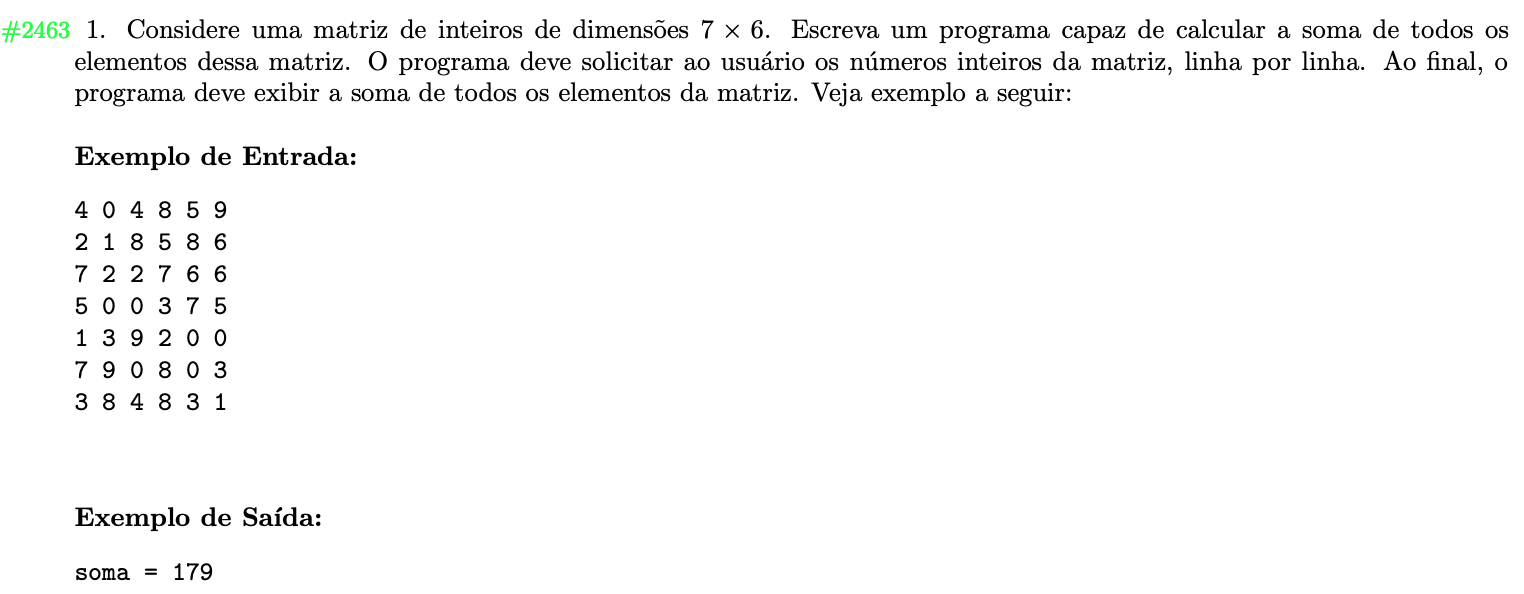
\includegraphics[width=0.9\textwidth]{cap10_questaoQT_EP_2_matriz.png}
  \caption{Recorte do PDF gerado para a questão de matriz definida nos Códigos \ref{lst:questaoQT_EP_2_matriz_parte1} e \ref{lst:questaoQT_EP_2_matriz_parte2}.}
  \label{fig:cap10_questaoQT_EP_2_matriz}
\end{figure}

\subsection{Criando as variações e imprimindo o PDF do exame}

Para criar um novo exame, siga os passos descritos no Capítulo \ref{ch:exames} -- \nameref{ch:exames}. Após definir o nome do exame, escolha a(s) turma(s), tópico(s) e as questões, preencha o restante da tela conforme apresentado na Figura \ref{fig:cap10_figExameVPL_Atualiza4}, realizando as devidas alterações nos campos  ``Dificuldade 1'', ``Dissertativa'' e ``Respostas/Questões/Ambos''. Finalize clicando no botão ``Salvar''.

\begin{figure}[htbp]
  \centering
  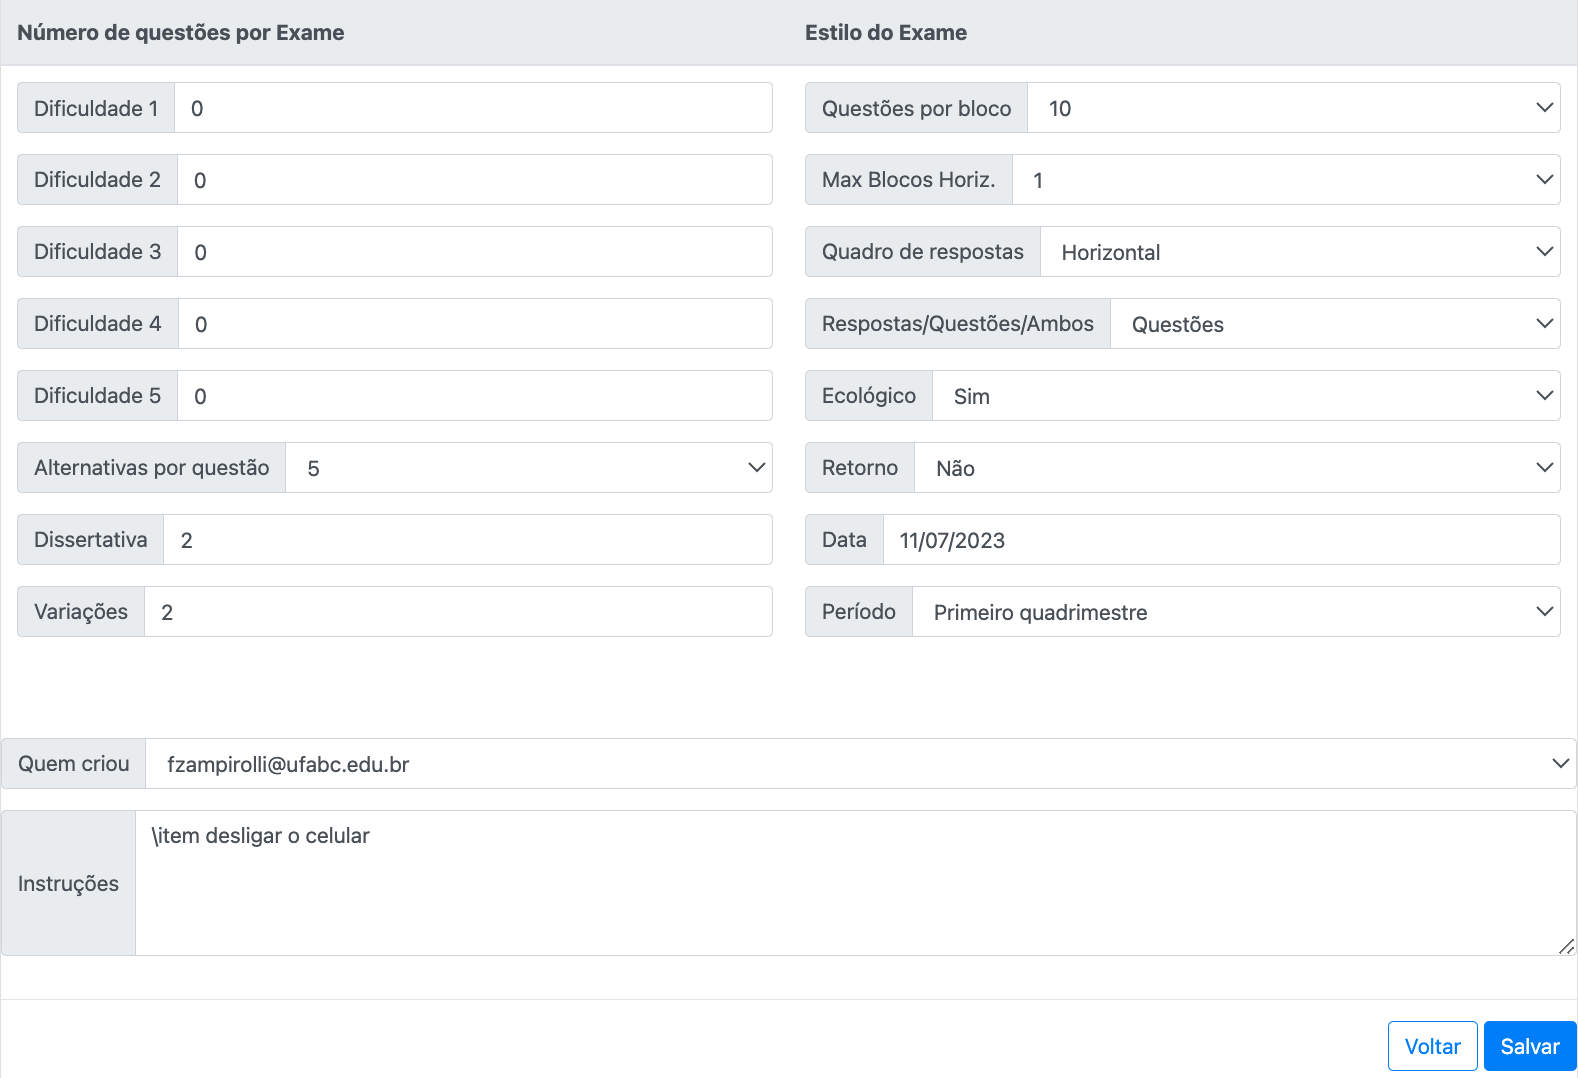
\includegraphics[width=0.9\textwidth]{cap10_figExameVPL_Atualiza4.png}
  \caption{Recorte da tela de exame, configurando os detalhes do exame com integração VPL.}
  \label{fig:cap10_figExameVPL_Atualiza4}
\end{figure}

Agora, para criar as variações, é importante selecionar a opção ``Json'' antes de clicar no botão ``Criar Variações'', conforme apresentado na Figura \ref{fig:cap10_exameVariacoes_detalhes}.

\begin{figure}[!ht]
  \centering
    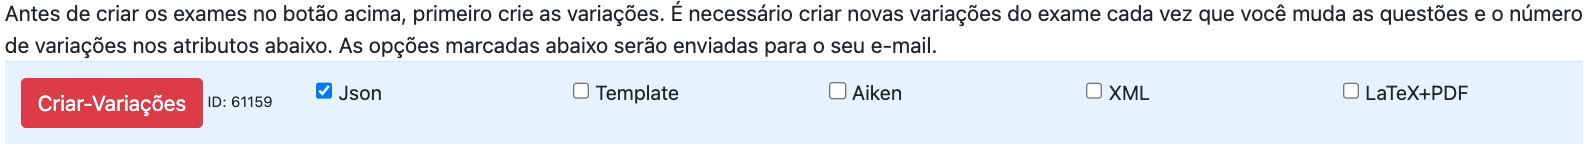
\includegraphics[width=0.9\textwidth]{cap10_exameVariacoes_detalhes.png}
    \caption{Recorte da tela do exame para criar as variações e enviar o arquivo no formato JSON.}
    \label{fig:cap10_exameVariacoes_detalhes}
  \end{figure}

Ao fazer isso, um arquivo no formato JSON com o nome \verb|*_linker.json| será gerado e enviado para o e-mail do professor. Esse arquivo deve ser renomeado para \verb|linker.json|. Veja na Figura \ref{fig:cap10_figExameVPL_email} o e-mail recebido, com remetente \verb|webmctest@ufabc.edu.br|. O arquivo JSON contém informações detalhadas sobre as variações do exame, incluindo as questões, as entradas utilizadas e as respostas esperadas.

\begin{figure}[htbp]
  \centering
  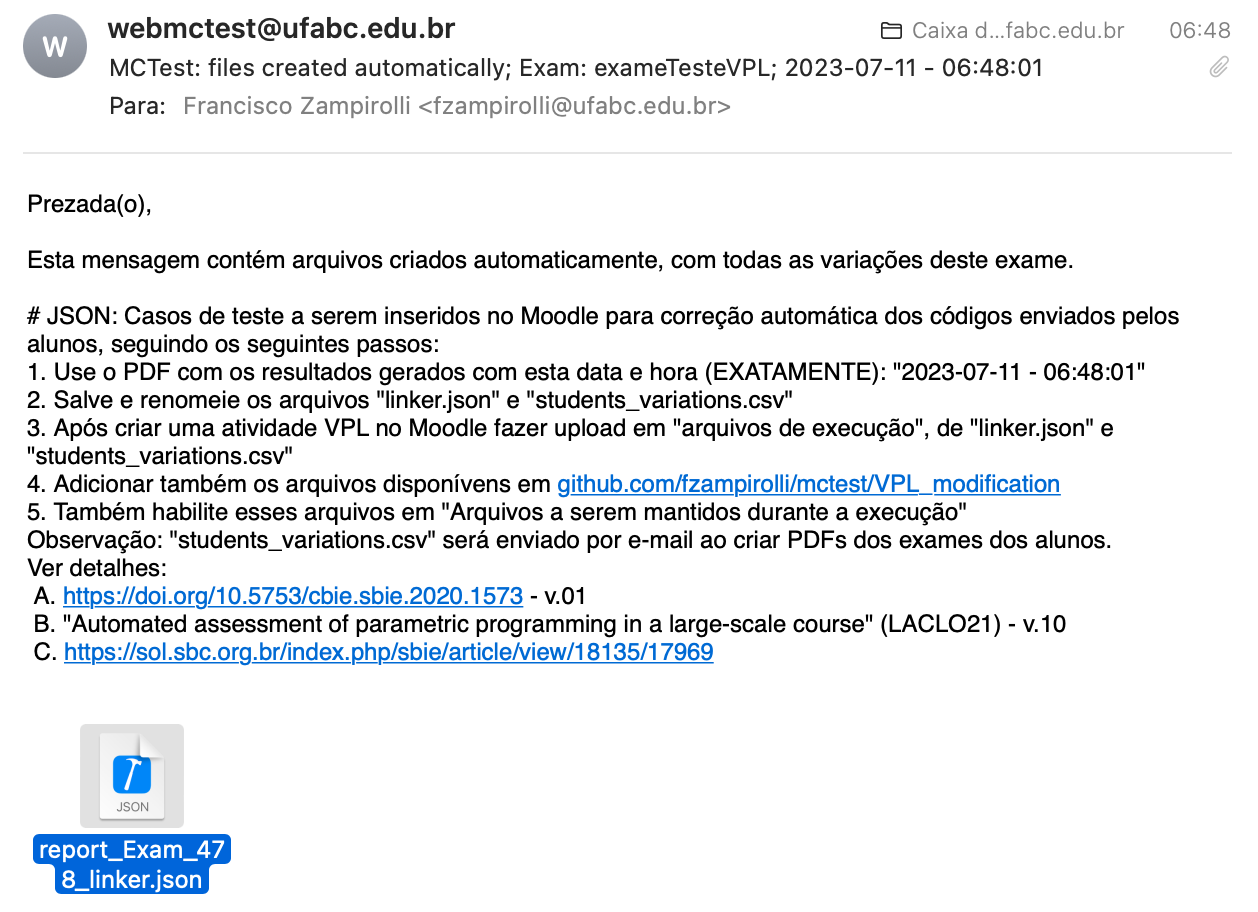
\includegraphics[width=0.9\textwidth]{cap10_figExameVPL_email.png}
   \caption{Recorte do e-mail recebido após clicar em ``Criar-Variações''.}
  \label{fig:cap10_figExameVPL_email}
\end{figure}

Após criar as variações, é possível gerar um PDF por turma contendo os exames dos estudantes. No entanto, antes de fazer isso, uma boa estratégia seria validar a atividade VPL no Moodle. Para isso, crie uma turma de teste incluindo somente o professor como estudante. Escolha essa turma no exame e, em seguida, clique no botão ``Criar-PDF''. Um PDF com o exame será enviado ao professor, conforme mostrado na Figura \ref{fig:cap10_figExameVPL_PDF}.
No mesmo e-mail, será anexado o arquivo \verb|*_students_variations.csv|, que deve ser renomeado para \verb|students_variations.csv|. Este arquivo contém as variações de cada estudante.

\begin{figure}[htbp]
  \centering
  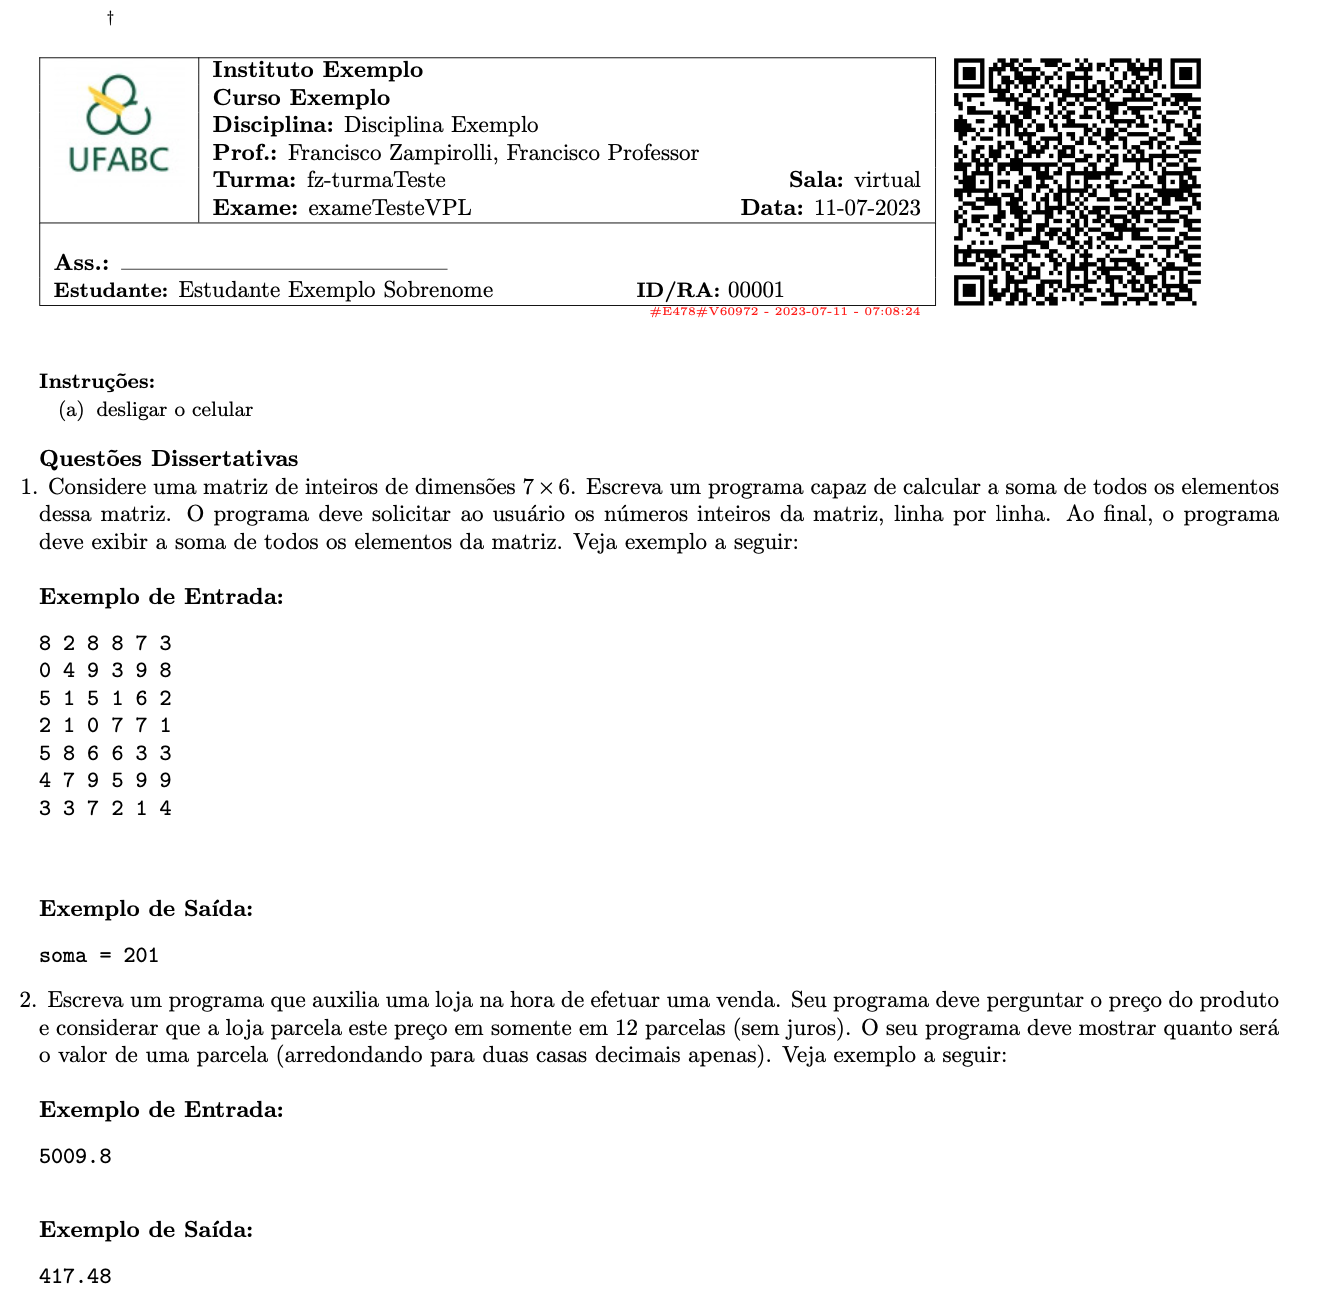
\includegraphics[width=0.9\textwidth]{cap10_figExameVPL_PDF.png}
  \caption{Recorte da tela do PDF do exame com integração VPL.}
  \label{fig:cap10_figExameVPL_PDF}
\end{figure}

\section{Criando e configurando a atividade VPL para o exame}

Adaptando as instruções definidas na Seção \ref{sec:questoesQT_VPL} -- \nameref{sec:questoesQT_VPL} para criar uma atividade VPL no Moodle:

\begin{enumerate}
    \item Acesse o Moodle e vá para a disciplina em que deseja adicionar um exame;
    \item Clique em ``Adicionar uma atividade ou recurso'' e selecione ``Laboratório Virtual de Programação'' para criar uma nova atividade VPL;

    \item Preencha os detalhes da atividade, como nome, descrição e pontuação. Em ``Número máximo de arquivos'', defina 2, pois o exame criado neste capítulo possui duas questões. Finalize salvando e mostrando a atividade. Em seguida, clique no ícone de engrenagem para acessar as configurações avançadas da atividade e siga os próximos passos;

    \item Na seção ``Opções de execução'', selecione a linguagem ``Python'' como ``Script de execução'', deixando apenas ``Avaliar'' e ``Atribuição automática de nota'' como ``Sim'', por exemplo;

    \item Na seção ``Arquivo de execução'', inclua os arquivos disponíveis na última versão disponível em \href{https://github.com/fzampirolli/mctest/tree/master/VPL_modification}{github.com/fzampirolli/mctest/tree/master/VPL\_modification/V13-Moodle\_v4.1}. 
    %Os arquivos para \textit{download} são: \verb|makefile|, \verb|vpl_evaluate.sh| e \verb|zip.tar.gz.b64|. 
    Inclua também os novos arquivos \verb|linker.json| e \verb|students_variations.csv|, que foram gerados recentemente pelos botões ``Criar-Variações'' e ``Criar-PDF'', respectivamente;

    \item Para que o Moodle selecione a variação correta do exame, é crucial que o endereço de e-mail seja idêntico tanto no Moodle quanto no arquivo \verb|students_variations.csv|; 

    \item Em ``Arquivos a serem mantidos durante a execução'', marque todas as opções e clique em Salvar;

    \item Para realizar a atividade do exame, clique na opção ``Atividade de teste'' e em seguida em ``Editar''. Será aberta uma janela solicitando o nome do arquivo, que deve ser exatamente \verb|Q1.py|. Caso utilize o nome \verb|q1.py|, a atividade não funcionará corretamente. Caso deseje criar um segundo arquivo, clique no ícone ``+'' e o ícone para criar um novo arquivo, em seguida utilize exatamente o nome do arquivo \verb|Q2.py|.
    
\end{enumerate}


\begin{mybox}{corEdicao2}{\textbf{Destaque:\\\vspace{-3mm}\hrule\vspace{3mm}}}
  \begin{enumerate}
    \item No item 6, na versão 5.3 do MCTest, o email foi incluído no arquivo \verb|students_variations.csv| como parte das informações do estudante, juntamente com o nome completo e a variação sorteada;
    \item Nas versões anteriores, a alteração do nome do estudante de \verb|Estudante Exemplo Sobrenome| para \verb|Francisco Exemplo Zampirolli|, conforme mostrado na Figura \ref{fig:cap10_figExameVPL_PDF}, era necessária porque a chave de busca era o Nome e Sobrenome do estudante;
    \item Agora, com a versão 5.3, a chave de busca é o email do estudante.
  \end{enumerate}  
\end{mybox}

\section{Soluções da atividade VPL para o exame}


Após criar os arquivos \verb|Q1.py| e \verb|Q2.py|, inclua soluções para resolver essas questões. Por exemplo, confira no Código \ref{lst:ExameVPLsolucaoQ1} uma solução para a primeira questão de matriz. A parte crítica desta questão é o estudante ter que ler 7 linhas, contendo 6 elementos em cada linha, conforme ilustrado na Figura \ref{fig:cap10_figExameVPL_PDF}. 


\begin{listing}[!ht]
\begin{myboxCode}{corCodigo}{\textbf{Questão: } }\vspace{3mm}
\hrule
\begin{minted}[xleftmargin=20pt,linenos=true]{python}
import numpy as np

# Definição das variáveis que indicam o número de linhas e colunas da matriz
linhas, colunas = 7, 6

# Inicialização da matriz M como uma lista vazia
M = []

# Loop para preenchimento da matriz M
for l in range(linhas):
    # Inicialização da linha l da matriz M como uma lista vazia
    linha = []
    
    # Leitura da linha l da matriz como uma string separada por espaços em branco
    linhaChar = input().split(' ')
    
    # Loop para preencher a linha l da matriz M com os valores lidos pelo usuário
    for c in linhaChar:
        # Verificação se o caractere não é vazio
        if c:
            # Conversão e inserção do valor na linha l da matriz M
            valor = int(c)
            linha.append(valor)
    
    # Adição da linha l à matriz M
    M.append(linha)

# Cálculo da soma de todos os elementos da matriz M utilizando o método sum 
soma = np.sum(M)

# Impressão do resultado da soma
print(f'soma = {soma}')
\end{minted}
\end{myboxCode}
\caption{Exemplo de solução para a questão de matriz do exame no VPL.}
\label{lst:ExameVPLsolucaoQ1}
\end{listing}

Uma solução mais concisa e genérica para a questão Q1 é apresentada no Código \ref{lst:ExameVPLsolucao2Q1}. É importante ressaltar que essa solução é viável porque todos os casos de teste gerarão entradas no mesmo formato, como exemplificado na Figura \ref{fig:cap10_figExameVPL_PDF}.

Essa solução consegue ler matrizes de quaisquer dimensões, caso possuam os mesmos tipos de elementos, que neste exemplo são inteiros, separados por espaços, e cada linha da matriz seja lida com apenas um comando \verb|input()|. Essa abordagem mais compacta permite uma maior legibilidade do código e pode ser útil em casos em que a entrada segue um formato padrão e bem definido.

No entanto, é importante ressaltar que essa solução pode não ser adequada para cenários em que a entrada varie em formato ou tamanho. Nesses casos, é mais indicado utilizar uma abordagem mais específica para a leitura da entrada. Além disso, é fundamental que o enunciado da questão seja claro e objetivo, permitindo que o estudante compreenda as restrições e especificações do problema. Dessa forma, o estudante poderá desenvolver uma solução adequada e eficiente, considerando todas as competências a serem avaliadas.

Por fim, é importante mencionar que a escolha da linguagem de programação pode impactar o desenvolvimento da solução, e que, portanto, é recomendável que o enunciado seja elaborado para permitir soluções em diferentes linguagens. Assim, os estudantes terão a oportunidade de aplicar seus conhecimentos e habilidades em diferentes contextos.

\begin{listing}[!ht]
\begin{myboxCode}{corCodigo}{\textbf{Questão: } }\vspace{3mm}
\hrule
\begin{minted}[xleftmargin=20pt,linenos=true]{python}
import numpy as np

def lerMatriz(): 
    """ler matriz de inteiros"""
    M, ler_linha = [], input()
    while ler_linha:
        M.append([int(i) for i in ler_linha.split(' ') if i])
        ler_linha = input()
    return M
  
print(f'soma = {np.sum(lerMatriz())}')
\end{minted}
\end{myboxCode}
\caption{Exemplo de solução compacta e genérica para a questão de matriz do exame no VPL.}
\label{lst:ExameVPLsolucao2Q1}
\end{listing}

A segunda questão sobre parcelas sem juros, a ser inserida no arquivo de código \verb|Q2.py| da atividade VPL, pode ser resolvida com o seguinte comando: \verb|print(f"{float(input())/12:.2f}")|. Este comando lê a entrada fornecida, converte para o formato \verb|float|, divide por 12 parcelas (como definido no enunciado da segunda questão na Figura \ref{fig:cap10_figExameVPL_PDF}) e formata o resultado com duas casas decimais.


\section{Detalhando o arquivo \texttt{linker.json}}

Esta seção detalha o arquivo \verb|linker.json|, sendo amplamente utilizado para trocar dados entre sistemas e fornece uma maneira fácil de armazenar e acessar informações estruturadas. Com o arquivo \verb|linker.json|, o professor pode facilmente importar as variações do exame em um sistema de gerenciamento de exames, como o Moodle com VPL, para criar e administrar o exame.

A versão mais recente, a 13, disponível no \href{https://github.com/fzampirolli/mctest/tree/master/VPL_modification/V13-Moodle_v4.1}{GitHub}, considera o arquivo \verb|linker.json| criado pela nova versão 5.3 do MCTest. Isso possibilita aproveitar todos os novos recursos ao criar uma questão no MCTest com integração VPL. Destaca-se a adição de uma nova chave no dicionário, chamada \verb|skills|. Essa chave contém um conjunto de habilidades que o estudante deve desenvolver para resolver a questão. Por exemplo, se a questão avalia a competência do estudante em criar laços de repetição utilizando o comando \verb|while|, as adaptações nos arquivos do VPL que devem ser incluídas verificarão se o estudante realmente utilizou essa habilidade. É importante ressaltar que para cada disciplina devem existir conjuntos específicos de habilidades a serem avaliadas e implementadas nestes arquivos VPL, e esses conjuntos devem crescer progressivamente. Essas implementações no VPL estão em processo de construção; no entanto, a estrutura necessária no arquivo JSON já está definida.

Dessa forma, o arquivo \verb|linker.json| se torna uma ferramenta valiosa para avaliar as competências dos estudantes de forma mais precisa e objetiva. Com as adaptações nos arquivos do VPL, é possível verificar se as habilidades necessárias para resolver a questão foram efetivamente utilizadas, garantindo uma avaliação mais coerente para aprendizagem da disciplina.

Na Seção \ \ref{sec:questao_VPL} -- \nameref{sec:questao_VPL}, \ é apresentado o dicionário \verb|moodle_cases| de uma QT com integração VPL para popular o arquivo \ \verb|linker.json|. O trecho de código a seguir exemplifica como o arquivo \verb|linker.json| é estruturado.

O arquivo JSON apresentado a seguir consiste em uma variação de questões do exame, identificada pela chave \verb|variant|, e uma lista de questões. Cada questão é identificada pela chave \verb|key|, sendo um valor único do banco de dados associado a cada questão. Além disso, a questão possui um número de identificação, indicado pela chave \verb|number|, que representa a ordem da questão na variante do exame, um arquivo de código relacionado, indicado pela chave \verb|file|, que deve ser utilizado com o mesmo nome e extensão em alguma linguagem, como \verb|Q1.py| para Python, e um peso, indicado pela chave \verb|weight|. Este peso é a dificuldade da questão, definida na Seção \ref{sec:questaoNavegacao} -- \nameref{sec:questaoNavegacao} (ver Figura \ref{fig:cap04_figQuestaoCria}). Por exemplo, se um exame tem duas questões VPL, com dificuldades 1 e 2, respectivamente, a primeira questão terá uma nota fracionada de 1/3, enquanto a segunda questão valerá 2/3, sendo que a segunda questão tem o dobro da dificuldade da primeira.


\begin{myboxCode}{corCSV}{\textbf{Conteúdo do arquivo linker.json até a primeira questão:}}\vspace{3mm}
  \hrule
  {\scriptsize 
  \begin{verbatim}
  {
    "variations": [
      {
        "variant": "1",
        "questions": [
          {
            "key": "2463",
            "number": "1",
            "file": "Q1",
            "weight": "1",
            "language": [
              "all"
            ],
            "skills": [],
            "answer": [],
            "description": [],
    ...
  \end{verbatim}
  }
  \end{myboxCode}
  
A questão também pode ter uma lista de linguagens de programação possíveis para a sua resolução, indicada pela chave \verb|language|, uma lista de habilidades que o estudante deve desenvolver para resolvê-la, indicada pela chave \verb|skills|, e uma descrição, indicada pela chave \verb|description|, que pode ser o enunciado da questão a ser apresentado na descrição da questão no Moodle em formato TXT. Por fim, a questão contém uma lista de casos de teste, cada um contendo uma entrada e uma saída esperada, indicados pelas chaves \verb|input| e \verb|output|, respectivamente.

Vale relembrar que a definição do arquivo JSON contou com a valorosa colaboração do Prof. Dr. Paulo Henrique Pisani e seu orientando Heitor Rodrigues Savegnago para a
adaptação dos arquivos de configuração do VPL.

Essa estrutura permite uma administração mais eficiente e precisa do exame, possibilitando a criação de diferentes variações de questões com pesos e habilidades diferentes.

% \tiny < \scriptsize < \footnotesize < \small < \normalsize < \large < \Large < \LARGE < \huge < \Huge

\begin{myboxCode}{corCSV}{\textbf{Continuação do conteúdo do arquivo linker.json até a primeira questão:}}\vspace{3mm}
  \hrule
  {\scriptsize 
  \begin{verbatim}
  {
  ...  
          "cases": [
            {
             "case": "test_1",
             "input": [
             "8 2 8 8 7 3\n0 4 9 3 9 8\n5 1 5 1 6 2\n2 1 0 7 7 1\n5 8 6 6 3 3\n4 7 9 5 9 9\n3 3 7 2 1 4\n\n"
              ],
             "output": [
               "soma = 201"
             ]
            },
            {
             "case": "test_2",
             "input": [
             "7 6 1 8 5 6\n1 6 2 4 2 3\n9 1 1 4 2 5\n1 9 5 8 1 3\n7 1 5 0 1 8\n2 8 2 0 0 2\n6 8 2 4 0 6\n\n"
              ],
             "output": [
               "soma = 162"
             ]
            }
          ]
        },
        ...
\end{verbatim}
}
\end{myboxCode}

A seguir, é apresentada a segunda questão da primeira variação do exame, seguindo a mesma ordem da questão anterior. Como mencionado anteriormente, essa estrutura permite que o arquivo \verb|linker.json| seja facilmente gerenciado e adaptado para diferentes necessidades, possibilitando a criação e administração de exames de forma mais eficiente e precisa. Dessa forma, é possível criar diferentes variações do exame, com questões e pesos diferentes, para avaliar as competências dos estudantes de forma mais abrangente.


\begin{myboxCode}{corCSV}{\textbf{Conteúdo do arquivo linker.json da segunda questão:}}\vspace{3mm}
\hrule
{\scriptsize 
\begin{verbatim}
        ...
        {
          "key": "2454",
          "number": "2",
          "file": "Q2",
          "weight": "1",
          "language": [
            "all"
          ],
          "skills": [],
          "answer": [],
          "description": [],

...
\end{verbatim}
}
\end{myboxCode}

\begin{myboxCode}{corCSV}{\textbf{Continuação do conteúdo do arquivo linker.json até a segunda questão:}}\vspace{3mm}
\hrule
{\scriptsize 
\begin{verbatim}
{
... 
          "cases": [
            {
              "case": "test_1",
              "input": [
                "5009.8\n"
              ],
              "output": [
                "417.48"
              ]
            },
            {
              "case": "test_2",
              "input": [
                "5009.7\n"
              ],
              "output": [
                "417.47"
              ]
            }
          ]
        }
      ]
    },
    ...
\end{verbatim}
}
\end{myboxCode}

\section{Considerações finais}

Neste capítulo, foi apresentado como criar exames integrados ao \textit{plugin} VPL do Moodle, contendo QTs paramétricas nas quais os estudantes devem submeter EP. Esse tipo de avaliação tem sido amplamente utilizado em disciplinas de cursos de graduação e pós-graduação da UFABC, principalmente nas disciplinas introdutórias envolvendo programação.

A integração do VPL com o Moodle permite a correção automática das atividades de programação submetidas pelos estudantes. Para isso, são necessários dois arquivos gerados pelo MCTest: o \verb|linker.json|, contendo as variações do exame e os detalhes de cada questão, principalmente os casos de teste; e o \verb|students_variations.csv|, contendo a variação atribuída a cada estudante. Esses arquivos devem ser inseridos na configuração da atividade VPL para a correção automática ocorrer. Foram detalhados todos os passos necessários para criar uma atividade VPL para um exame, incluindo a configuração dos arquivos citados.

O arquivo \verb|linker.json| é uma ferramenta essencial para transferir dados entre sistemas, contendo de maneira estruturada todas as informações de um exame, como variações de questões, descrições, pesos, habilidades, casos de teste, entre outros. A versão mais atual desse arquivo está sendo validada e em breve será disponibilizada, contendo novas chaves como \verb|skills|, que especifica as habilidades que o estudante deve desenvolver para resolver cada questão. Isso permite uma avaliação mais precisa das competências dos estudantes.

Apesar dos benefícios da avaliação por meio de atividades práticas na aprendizagem ativa, muitos docentes ainda não utilizam essa metodologia. A adoção de exames padronizados, como os apresentados neste trabalho, pode auxiliar na uniformização dos conteúdos e habilidades desenvolvidas pelos estudantes, fortalecendo o processo de ensino-aprendizagem. 

Conclui-se esta parte sobre a criação e correção de exames de diferentes estilos, incluindo quadros de respostas (QRs), além de QMs e QTs. Estas últimas podem conter EP que são passíveis de correção automática utilizando o \textit{plugin} VPL do Moodle. Espera-se que, até este ponto do livro, o potencial do MCTest para criar e corrigir exames tenha sido evidenciado ao professor. Para comprovar seus benefícios, nos próximos capítulos serão apresentados resumos dos principais resultados publicados até o momento.

